\chapter{Radio-goniométrie}



Dans cette partie, nous allons nous attacher à étudier les différents types de goniométrie existant afin de retenir la solution la plus pertinente pour notre système. Cette étude redéfinira dans un premier temps le cadre de l’étude, puis suivra une explication de chaque technologie existante afin de conclure sur le choix que nous aurons retenu.
~\\

Généralement, un système de radiogoniométrie est composé de  :

\begin{itemize}
\item Un réseau de N capteurs avec ou sans processus de mise en forme des signaux d’antennes.

\item Un commutateur d’antenne
\item Un récepteur à plusieurs voies
\item Une unité de traitement du signal

\end{itemize}
~\\
De plus, la composition du système d’acquisition et les techniques de traitement du signal dépendent :
\begin{itemize}
\item  Des caractéristiques de l’onde à étudier
\item  Du type d’acquisition de l’information
\end{itemize}
~\\
Dans notre application, le système devra détecter une onde émise dans la gamme de fréquence UHF (2,4 GHz). Bien qu’existant dans le domaine de réalisation des radiogoniomètres, il n’est pas commun qu’un radiogoniomètre travail sur cette gamme de fréquence.

Les caractéristiques principales qui interviennent principalement dans le choix d’un radiogoniomètre sont:

\begin{itemize}
\item La précision de mesure angulaire (précision de la position obtenue)
\item La sensibilité (portée maximale du système) 
\item La vitesse de mesure
\item Le comportement en présence de plusieurs ondes dans la bande d’analyse
\item La susceptibilité du système
\end{itemize}
~\\
La spécificité de notre système est la cible à localisé. En effet, la source peut ne pas émettre en  continue et sur de très courtes période (inférieure à 1 seconde). Il nous faut donc un radiogoniomètre capable de réalisé la mesure en une fraction de seconde. La gestion de conservation de la donnée mesurée en attendant une valeur ultérieure sera gérée par l’ordinateur.


\section{Type de goniométrie}

\subsection{Goniométrie d'amplitude}

	La mesure se fait par repérage d’un maximum d’amplitude, d’un minimum d’amplitude, ou par comparaison de d’amplitude en sortie de deux diagrammes se recouvrant partiellement. La recherche du minimum d’amplitude à partir d’une antenne à cadre tournante est l’approche la plus ancienne. Un dipôle électrique est utilisé pour lever l’ambiguïté de 180◦ en formant un diagramme en cardioïde par sommation.
	
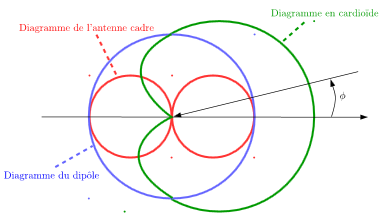
\includegraphics[width=\textwidth]{cardioide}
\captionof{figure}{diagramme en cardioide d’une antenne à cadre}
\parindent=15pt

	La formation de faisceaux est une technique plus récente issue des traitements radar. Elle utilise un ensemble de capteurs spatialement répartis. Les sorties d’antennes sont pondérées en phase puis sommées. Cette pondération est fonction du déphasage progressif d’une antenne à une autre, qui dépend de la direction d’arrivée et de la distance entre capteurs. Les pondérations permettent ainsi de remettre en phase les signaux et d’obtenir un diagramme avec un maximum dans la direction d’arrivée.
 Cette technologie est la plus ancienne. L’antenne utilisée était une antenne cadre et la gamme de fréquence étudiée était la HF et la VHF.

\subsection{Goniométrie Watson-Watt}

	Un radiogoniomètre Watson-Watt est un radiogoniomètre automatique. L’onde électromagnétique du système à localisé est reçue par deux antennes perpendiculaires dont le rapport des amplitudes est très proche de tan (l’une en sin et l’autre en cos). La goniométrie par interférométrie est considérée comme une technique plus performante comparée à celles citées précédemment. A la différence des deux techniques précédentes, le traitement n’est pas entièrement analogique. Des calculs numériques, plus ou moins complexes, sont nécessaires suivant la topologie de l’antenne utilisée. Elle n’a donc pu être mise en œuvre qu’à partir de l’arrivée des microprocesseurs.

\subsection{Goniométrie par interférométrie}

	La goniométrie par interférométrie est considérée comme une technique plus performante comparée à celles citées précédemment. A la différence des deux techniques précédentes, le traitement n’est pas entièrement analogique. Des calculs numériques, plus ou moins complexes, sont nécessaires suivant la topologie de l’antenne utilisée. Elle n’a donc pu être mise en œuvre qu’à partir de l’arrivée des microprocesseurs.
L’interférométrie utilise la mesure de la différence de phase de signaux délivrés par deux antennes proches illuminées par la même onde électromagnétique.

\subsection{Goniométrie par effet Doppler}

	Une antenne tournant autour d'un axe est placé dans le champ d'émission d'un émetteur de porteuse pure. A cause du mouvement de l'antenne, le signal reçu subit un effet Doppler qui se traduit par une modulation FM du signal reçu. La fréquence instantanée du signal augmente quand l’antenne se rapproche de la direction d’arrivée du signal et décroît lorsqu’elle s’en éloigne. En effectuant une démodulation FM, on peut détecter la direction de provenance des ondes en comparant la phase du signal obtenu et celle de la rotation angulaire de l’antenne. 
Afin d'éviter de devoir faire tourner mécaniquement l'antenne, on peut en disposer plusieurs en cercle et les commuter successivement.

\section{Selection de la technologie}

	Après étude des différentes technologies existantes, nous nous baserons sur une étude comparative menée par le site F1LVT.

~\\	
	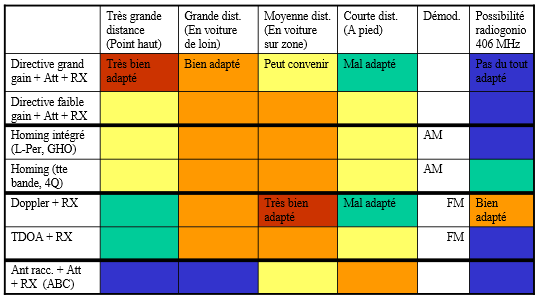
\includegraphics[width=\textwidth]{tableauTechnologies}
	\captionof{figure}{Radiogoniométrie VHF-UHF pour les bandes aviation et les bandes RA}
\parindent=15pt
~\\

	Ce tableau compare plusieurs technologies ainsi que leurs caractéristiques. Dans le cadre d’un système devant opéré en extérieur sur zone (environ de zone industriel ou de central électrique ) nous retenons le goniomètre Doppler.





%%% Local Variables: 
%%% mode: latex
%%% TeX-master: "rapport_analyse"
%%% End:
